\documentclass[11p]{article}
% Packages
\usepackage{amsmath}
\usepackage{graphicx}
\usepackage{fancyheadings}
\usepackage[swedish]{babel}
\usepackage[
    backend=biber,
    style=authoryear-ibid,
    sorting=ynt
]{biblatex}
\usepackage[utf8]{inputenc}
\usepackage[T1]{fontenc}
\usepackage{hyperref}
\usepackage[exprot]{adjustbox}
%Källor
\addbibresource{references.bib}
\graphicspath{ {./images/} }

% Lite variabler
\def\email{Fabian.Sigfridsson@ga.ntig.se}
\def\foottitle{Bakgrund}
\def\name{Fabian Sigfridsson}

\title{Bakgrund \\ \small Gymnasiearbete}
\author{\name}
\date{\today}

\begin{document}
% fixar sidfot
\lfoot{\footnotesize{\name \\ \email}}
\rfoot{\footnotesize{\today}}
\lhead{\sc\footnotesize\foottitle}
\rhead{\nouppercase{\sc\footnotesize\leftmark}}
\pagestyle{fancy}
\renewcommand{\headrulewidth}{0.2pt}
\renewcommand{\footrulewidth}{0.2pt}

% i Sverige har vi normalt inget indrag vid nytt stycke
\setlength{\parindent}{0pt}
% men däremot lite mellanrum
\setlength{\parskip}{10pt}

\maketitle

\section{Bakgrund}
Transmission, också kallad växellåda, är en mekanisk enhet som använder kugghjul för att ändra hastighet och/eller rotationsriktning.
En transmission kan ha flera olika utväxlingar, men det finns också dom med bara en utväxling.
Sammansatta transmissionssystem är när man har flera enkla transmissionsenheter sammansatta i en enhet.
Vridmoment är ett mått på en krafts förmåga att snurra på ett objekt kring en axel.
Vridmoment beror på både längden av hävarmen och kraften på hävarmen.
Enheten för vridmoment betecknas ofta i newton meter (Nm).
Växellådor eller i det här fallet momentomvandlare är något som tar ett vridmoment och ändrar hastigheten och kraften, oftast att man minskar hastigheten och att kraften då blir större.
En momentomvandlare kan ha olika typer av mekanisk omvandling, det kan vara kugghjulsväxel, planetväxel och snäckväxel mm.
En kugghjulsväxel fungerar så att ett kugghjul har mer tänder (kuggar) än det andra vilket gör så att om ett hjul snurrar ett varv så har det andra antingen snurrat mer eller mindre än det första.
En planetväxel är ett sammansatt transmissionssystem som består av kugghjul.
\begin{figure}[ht]
    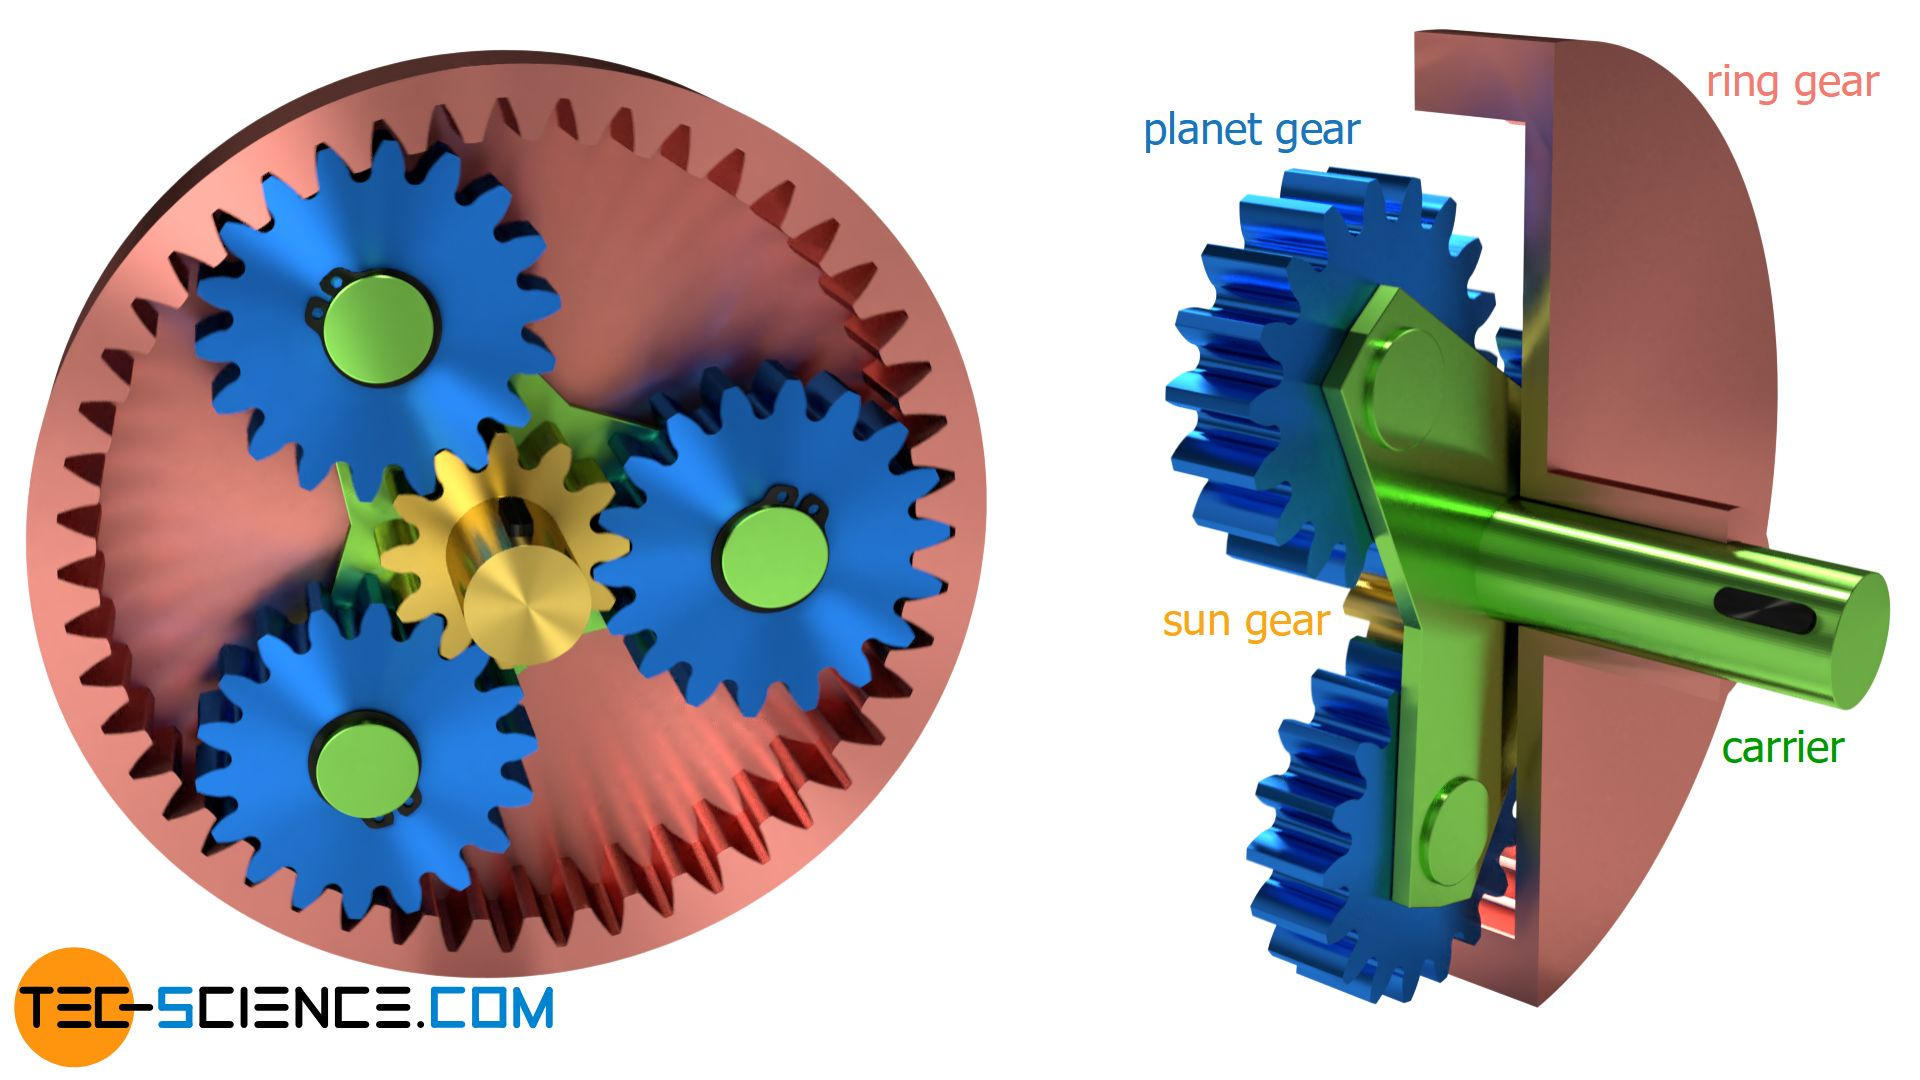
\includegraphics[width=0.8\textwidth]{planetary_gearbox.jpg}
    \caption{Planetväxel}
    \label{fig:planet}
\end{figure}

Det finns tre typer av planetväxlar.
Varianternas skillnader är vilka av hjulen som snurrar.
Den variant som kommer undersökas fungerar så att solhjulet är ingången, den som drivs av motorn, planethjulen är sammankopplade av en carrier och är utgången och ringhjulet är stationärt.
När solhjulet snurrar så kommer planethjulen att gå runt solhjulet och göra så att carriern börjar snurra.
Efter som att planethjulen inte kan snurra ett helt varv i ringhjulet på ett varv av solhjulet så kommer carriern att ha en lägre hastighet än solhjulet.

En snäckväxel består av två delar, ett kugghjul och en snäckskruv (skruv).
\begin{figure}[!h]
    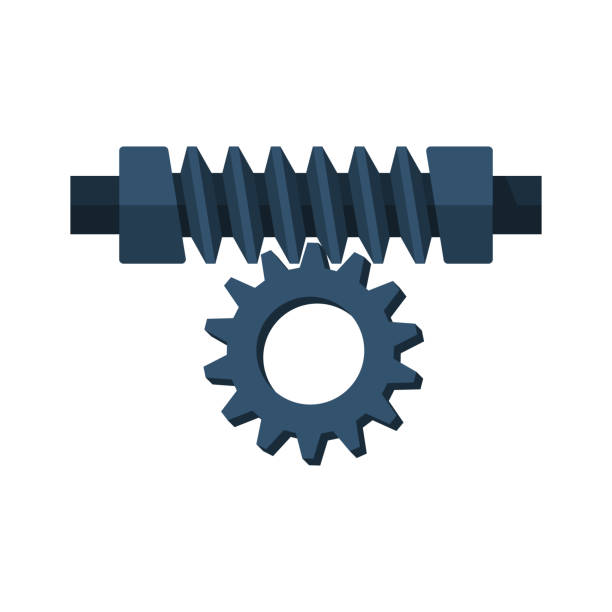
\includegraphics[width=0.8\textwidth]{snäckväxel.jpg}
    \caption{Snäckväxel}
    \label{fig:snäck}
\end{figure}

Den fungerar så att skruven är fäst till ingång och kugghjulet är utgång.
När man snurrar på skruven så puttar den på kuggarna på kugghjulet vilket gör att den börjar snurra.
Eftersom att ett varv på skruven inte kommer att putta på alla kuggarna på kugghjulet så kommer kugghjulet snurra långsammare än skruven.

Den typ av tredimensionella (3D) printer som kommer att användas är en typ av maskin som använder tillverkningsprincipen fused filament fabrication (FFF) som är en typ av additiv tillverkning (AM).
AM är en tillverknings princip där man bygger en del genom att lägga till material.
FFF, också känd som fused deposition modeling (FDM), är en metod av tillverkning där man har materialet (filament) i form av tråd, som oftast är på en spole. \textcite{3D_printable}
Metoden går ut på att filamentet går in i matare som trycker vidare filamentet in i en värmare och sen vidare ut genom ett munstycke till på byggplattan.
\begin{figure}[!h]
    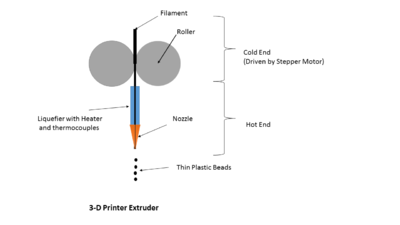
\includegraphics[width=0.8\textwidth]{3D_Printer_Extruder.png}
    \caption{Extruder}
    \label{fig:extruder}
\end{figure}

Filamentet som används är polylaktid (PLA).
PLA är en naturligt nedbrytningsbar termoplast.
PLA tillverkas från förnybara resurser, vanliga råvaror är bland annat rörsocker och majsstärkelse.

Referenser i text kan skrivas på två sätt: Enligt \textcite{} kan man använde två typer av referenser, inbäddade i texten eller ``efter'' ett fakta \parencite{Fraenkel}. Ett till test för att se hur det ser ut \parencite{fermi}.

\section{Annat som kan vara bra att veta}
Det är lätt att skriva matematik i \LaTeX

\begin{equation}
    F = G \frac{M m}{r^2}
    \label{eq:grav}
\end{equation}

Ekvation \eqref{eq:grav} känner ni igen...
\clearpage
\subsection{En underrubrik}
    \begin{figure}[!h]
        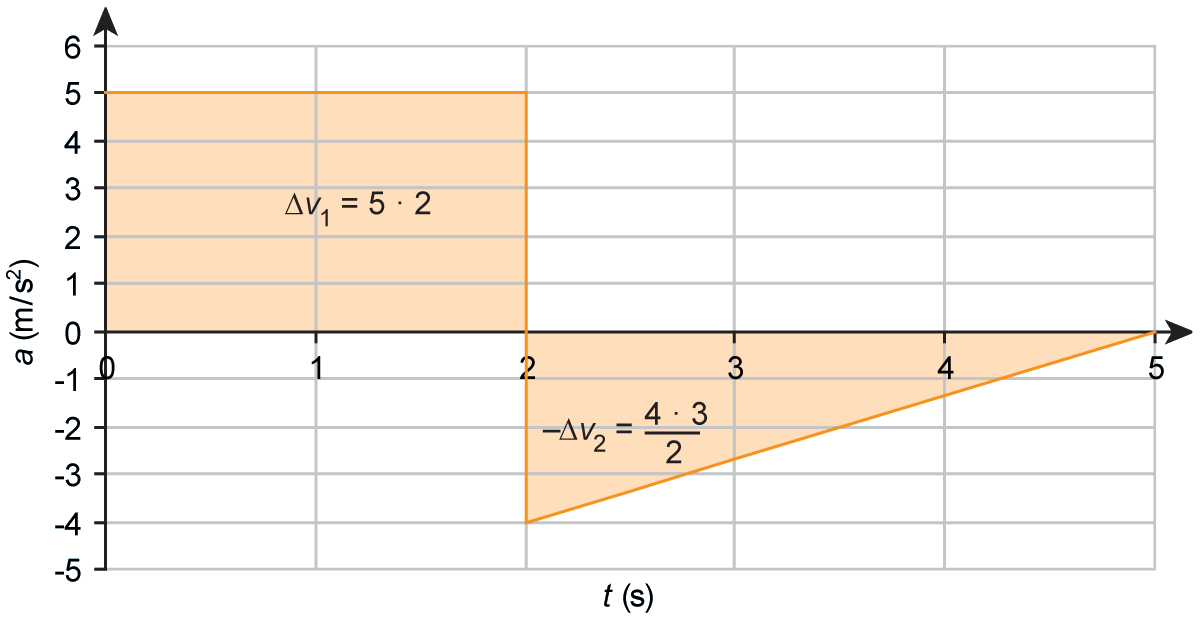
\includegraphics[width=0.8\textwidth]{accelerationTime.png}
        \caption{Acceleration-tid diagram. Källa: \textcite{Fraenkel}}
        \label{fig:acc}
    \end{figure}

Acceleration-tiddiagram (se figur \ref{fig:acc})

\printbibliography

\end{document}
